% !TEX root = ../slides.tex
%%%%%%%%%%%%%%%%%%%%%%%%%%%%%%%%%%%%%%%%%%%%%%%%%%%%%%%%%%%%%%%%%%%%%%%%%%%%%%%%
% Session 10: Orthogonal polynomials
%%%%%%%%%%%%%%%%%%%%%%%%%%%%%%%%%%%%%%%%%%%%%%%%%%%%%%%%%%%%%%%%%%%%%%%%%%%%%%%%

\session{session10}{Spectral methods}{Orthogonal polynomials}
{Sections 6.2--6.5}
{\notebook{lectures/spectral/basis}{interpolationerror.ipynb}}
{--}

\begin{frame}{Plan for today}
    \begin{enumerate}
        \item Sturm--Liouville problems and orthogonal polynomials.
        \item Polynomial interpolation: Lebesgue constant, Chebyshev nodes, Runge's phenomenon.
        \item Gauss and Gauss--Lobatto quadrature.
        \item Legendre polynomials.
        \item Chebyshev polynomials.
    \end{enumerate}
    \bigskip
    \takeaway{For non-periodic problems in $(-1,1)$ we replace $e^{ikx}$ by orthogonal polynomials, and the uniform grid by the zeros of these polynomials.}
\end{frame}

\begin{frame}{Sturm--Liouville problems}
    \small
    \[
        \tag{SL}
        -\big(p\, u'\big)' + q u = \lambda\, w\, u \quad \text{in } (-1,1), \qquad + \text{ suitable boundary conditions},
    \]
    with $p \in C^1$, $p > 0$ in $(-1,1)$; $q \ge 0$ bounded; weight $w \ge 0$ integrable; $\lambda$ the eigenvalue.
    \begin{lemma}[Singular case $p(\pm1) = 0$]
        If $u_\lambda, u_\mu \in C^2([-1,1])$ are eigenfunctions with $\lambda \ne \mu$, then
        \(
            (u_\lambda, u_\mu)_w \defeq \int_{-1}^1 u_\lambda u_\mu w = 0.
        \)
    \end{lemma}
    \begin{proofsteps}
        \begin{enumerate}
            \item Integrate by parts: $-\int_{-1}^1 (pu')'v = -\big[p u' v\big]_{-1}^{1} + \int_{-1}^1 p u' v' = \int_{-1}^1 p u'v'$, since $p(\pm 1) = 0$.
            \item The operator is symmetric, so
                  $\lambda (u_\lambda, u_\mu)_w = \int \big(-(pu_\lambda')' + qu_\lambda\big) u_\mu = \int u_\lambda \big(-(pu_\mu')' + qu_\mu\big) = \mu (u_\lambda, u_\mu)_w$.
        \end{enumerate}
    \end{proofsteps}
    \takeaway{No boundary conditions are needed: the degeneracy of $p$ at $\pm1$ does the job.}
\end{frame}

\begin{frame}{Orthogonal polynomials}
    Weight $w > 0$ a.e., integrable: \ $(u,v)_w = \int_{-1}^1 u v w$, \ $\|u\|_w = (u,u)_w^{1/2}$.
    \begin{itemize}
        \item Gram--Schmidt on $1, x, x^2, \dots$ gives orthogonal polynomials $p_k$ with $\deg p_k = k$.
        \item Coefficients and projection:
              \[
                  \hat u_k = \frac{(u, p_k)_w}{\|p_k\|_w^2}, \qquad P_N u = \sum_{k=0}^N \hat u_k p_k .
              \]
        \item Characterisation: $(P_N u, v)_w = (u,v)_w$ for all $v \in \R_N[x]$ (orthogonal projection onto $\R_N[x]$).
        \item Completeness (Weierstrass): $\|u - P_N u\|_w \to 0$ for every $u \in L^2_w(-1,1)$.
    \end{itemize}
\end{frame}

\begin{frame}{Polynomial interpolation}
    Given $N+1$ distinct nodes $x_0, \dots, x_N$: \ $I_N : C([-1,1]) \to \R_N[x]$, \ $I_N u(x_j) = u(x_j)$.
    \begin{definition}[Lebesgue constant]
        \[
            \Lambda_N = \sup_{v \ne 0} \frac{\|I_N v\|_{L^\infty}}{\|v\|_{L^\infty}} = \max_{x \in [-1,1]} \sum_{j=0}^N |L_j(x)|,
        \]
        where $L_j$ are the Lagrange polynomials of the nodes.
    \end{definition}
    \begin{remark}[Why $\Lambda_N$ matters]
        Since $I_N p = p$ for $p \in \R_N[x]$,
        \[
            \|u - I_N u\|_\infty \le \|u - p\|_\infty + \|I_N(p - u)\|_\infty \le (1 + \Lambda_N) \inf_{p \in \R_N[x]} \|u - p\|_\infty .
        \]
        $\Lambda_N$ grows exponentially for equi-distant nodes, but only like $\frac{2}{\pi}\log N$ for Chebyshev nodes.
    \end{remark}
\end{frame}

\begin{frame}{Interpolation error and Chebyshev nodes}
    \small
    For $u \in C^{N+1}([-1,1])$:
    \[
        \|u - I_N u\|_{L^\infty} \le \frac{[u]_{W^{N+1,\infty}}}{(N+1)!} \max_{x \in [-1,1]} \prod_{k=0}^N |x - x_k| .
    \]
    Equi-distant nodes: \ $\|u - I_N u\|_{L^\infty} \le \frac{2^{N-1}}{(N+1)N^{N+1}} [u]_{W^{N+1,\infty}}$.
    \begin{theorem}[Chebyshev nodes]
        For $x_k = \cos\frac{(2k+1)\pi}{2N+2}$, $k = 0, \dots, N$: \quad
        $\displaystyle \|u - I_N u\|_{L^\infty} \le \frac{1}{2^N (N+1)!} [u]_{W^{N+1,\infty}}$.
    \end{theorem}
    \begin{proofsteps}
        \begin{enumerate}
            \item The $x_k$ are the roots of $T_{N+1}(x) = \cos((N+1)\arccos x)$.
            \item Same roots, and leading coefficients $1$ and $2^N$: \ $\prod_{k}(x - x_k) = 2^{-N}\, T_{N+1}(x)$, and $|T_{N+1}| \le 1$.
        \end{enumerate}
    \end{proofsteps}
\end{frame}

\begin{frame}{Runge's phenomenon}
    \begin{columns}[c]
        \begin{column}{.5\textwidth}
            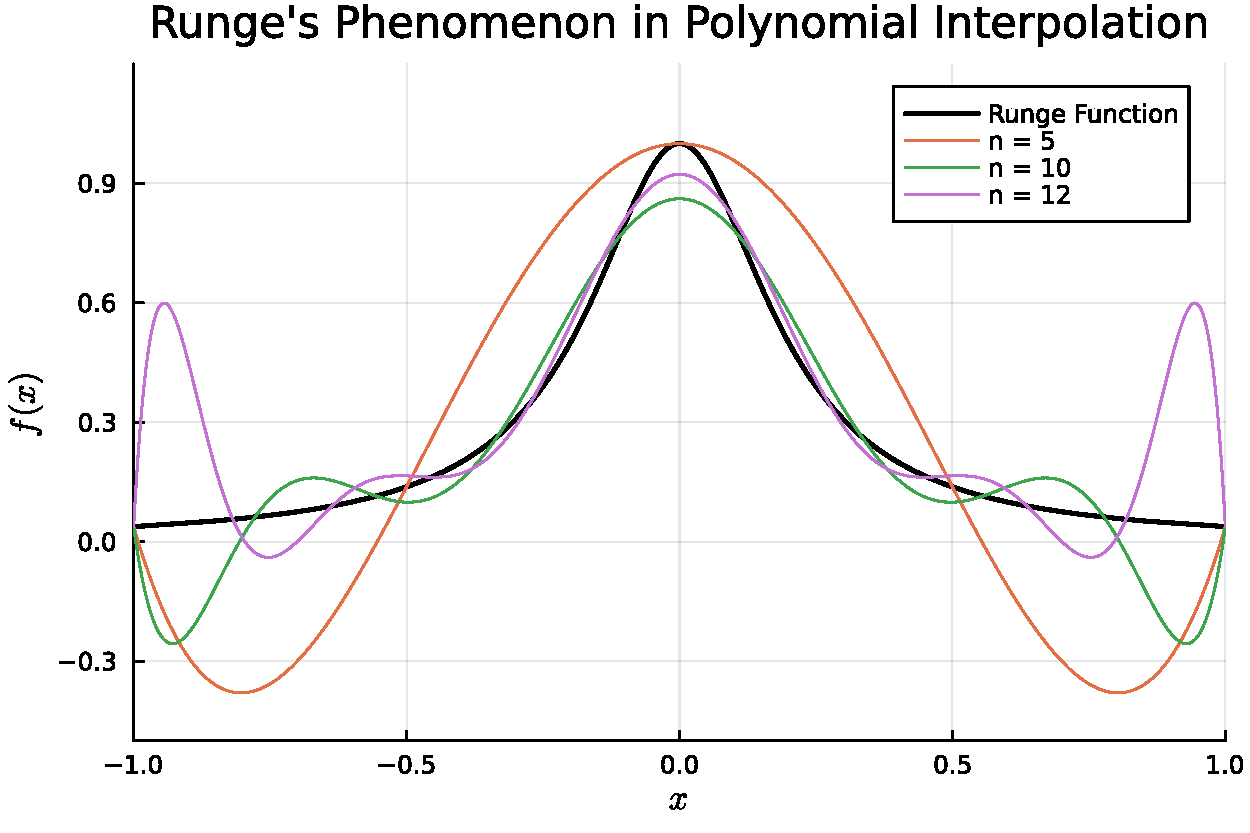
\includegraphics[width=\textwidth]{../../lectures/spectral/basis/Runge.pdf}
        \end{column}
        \begin{column}{.48\textwidth}
            Interpolation of $f(x) = \dfrac{1}{1 + 25x^2}$ at equi-distant nodes.
            \medskip

            The interpolants oscillate near $\pm1$ and do \alert{not} converge uniformly. Two reasons:
            \begin{enumerate}
                \item $f^{(n)}$ grows very fast with $n$;
                \item for equi-distant nodes the factor $\max \prod_k |x - x_k|$ does not decay fast enough.
            \end{enumerate}
            \medskip
            Remedies: choose the nodes wisely (Chebyshev), or use weights that are singular at $\pm1$, like $w = (1-x^2)^{-1/2}$.
        \end{column}
    \end{columns}
\end{frame}

\begin{frame}{Gauss quadrature}
    \small
    \begin{theorem}[Gauss quadrature]
        Let $p_k$ be orthogonal in $L^2_w(-1,1)$, $x_0, \dots, x_N$ the roots of $p_{N+1}$, and $w_j$ such that the rule is exact for $x^k$, $0 \le k \le N$. Then $w_j > 0$ and
        \[
            \sum_{j=0}^N p(x_j) w_j = \int_{-1}^1 p(x) w(x) \diff x \qquad \forall p \in \R_{2N+1}[x].
        \]
        No choice of $N+1$ nodes and weights is exact on $\R_{2N+2}[x]$.
    \end{theorem}
    \begin{proofsteps}
        \begin{enumerate}
            \item Divide: $p = q\, p_{N+1} + r$ with $q, r \in \R_N[x]$.
            \item $\int q\, p_{N+1} w = 0$ (orthogonality), and $q\,p_{N+1}$ vanishes at the nodes. The rule is exact for $r$.
            \item Positivity: apply the rule to $L_j^2 \in \R_{2N}[x]$: \ $w_j = \int L_j^2 w > 0$.
            \item Optimality: $\prod_j (x - x_j)^2 \in \R_{2N+2}[x]$ has zero sum but positive integral.
        \end{enumerate}
    \end{proofsteps}
\end{frame}

\begin{frame}{Gauss--Lobatto quadrature}
    For boundary-value problems we want the end points $\pm1$ among the nodes.
    \begin{theorem}[Gauss--Lobatto with Jacobi weights]
        Let $w_{\alpha,\beta}(x) = (1-x)^\alpha(1+x)^\beta$, $\alpha, \beta > -1$, with orthogonal (Jacobi) polynomials $J_k^{(\alpha,\beta)}$. Take
        \[
            x_0 = -1, \quad x_N = 1, \quad x_1, \dots, x_{N-1} \text{ the zeros of } \tfrac{\diff}{\diff x} J_N^{(\alpha,\beta)},
        \]
        and $w_j$ such that the rule is exact on $\R_N[x]$. Then
        \[
            \sum_{j=0}^N p(x_j) w_j = \int_{-1}^1 p(x)\, w_{\alpha,\beta}(x) \diff x \qquad \forall p \in \R_{2N-1}[x].
        \]
    \end{theorem}
    \begin{itemize}
        \item We lose two degrees of exactness ($2N-1$ instead of $2N+1$) because two nodes are fixed.
        \item Differentiation: $\mat D_N$ maps nodal values to the values of $\frac{\diff}{\diff x} I_N u$, and $\mat D_N^{(2)} = \mat D_N^2$.
    \end{itemize}
\end{frame}

\begin{frame}{Legendre polynomials}
    \small
    Sturm--Liouville with $p = 1 - x^2$, $q = 0$, $w = 1$:
    \[
        -\big((1-x^2) L_k'\big)' = k(k+1) L_k, \qquad L_k(1) = 1 .
    \]
    \begin{itemize}
        \item $L_0 = 1$, \ $L_1 = x$, \ $L_2 = \frac12(3x^2 - 1)$, \dots \ orthogonal in $L^2(-1,1)$, $\|L_k\|^2_{L^2} = \frac{2}{2k+1}$.
        \item \textbf{Legendre--Gauss:} $x_j$ zeros of $L_{N+1}$, \ $w_j = \dfrac{2}{(1 - x_j^2)\, L_{N+1}'(x_j)^2}$.
        \item \textbf{Legendre--Gauss--Lobatto:} $x_0 = -1$, $x_N = 1$ and the zeros of $L_N'$, \ $w_j = \dfrac{2}{N(N+1)} \dfrac{1}{L_N(x_j)^2}$.
    \end{itemize}
    \textbf{Approximation} ($u \in H^m(-1,1)$, $m \ge 1$):
    \[
        \|u - P_N u\|_{L^2} \le C N^{-m} \|u\|_{H^m},
        \qquad
        \|u - I_N u\|_{L^2} \le C N^{-m}\|u\|_{H^m},
    \]
    ($I_N$ at Gauss or Gauss--Lobatto nodes), and for the $H^1$-orthogonal projection $\Pi^1_N$:
    \(
        \|u - \Pi^1_N u\|_{H^1} \le C N^{1-m}\|u\|_{H^m}.
    \)
\end{frame}

\begin{frame}{Example: Legendre--Galerkin}
    \[
        -\big((1-x^2) u'\big)' = f \quad \text{in } (-1,1), \qquad f \in L^2(-1,1)
    \]
    (with the natural flux conditions $(1-x^2)u'(x) \to 0$ as $x \to \pm1$).
    \medskip

    Expand $u = \sum_k \hat u_k L_k$, multiply by $L_k$ and integrate by parts:
    \[
        k(k+1)\, (u, L_k) = (f, L_k).
    \]
    \begin{itemize}
        \item $k = 0$: compatibility condition $\int_{-1}^1 f = 0$; $u$ is unique up to constants (fix $\hat u_0 = 0$).
        \item Exact solution: \ $u = \sum_{k \ge 1} \frac{(f, L_k)}{k(k+1)\|L_k\|^2} L_k$.
        \item Galerkin in $V_N = \{v \in \R_N[x] : \int_{-1}^1 v = 0\}$ gives exactly $u_N = P_N u$.
    \end{itemize}
    \takeaway{As with Fourier: the basis diagonalises the operator.}
\end{frame}

\begin{frame}{Chebyshev polynomials}
    Sturm--Liouville with $p = \sqrt{1-x^2}$, $q = 0$, $w = (1 - x^2)^{-\frac12}$:
    \[
        -\big(\sqrt{1-x^2}\, T_k'\big)' = \frac{k^2}{\sqrt{1-x^2}} T_k,
        \qquad
        T_k(x) = \cos(k \arccos x).
    \]
    \begin{itemize}
        \item Recurrence: $T_0 = 1$, $T_1 = x$, $T_{n+1} = 2x T_n - T_{n-1}$ (leading coefficient $2^{n-1}$).
        \item The singular weight gives more importance to $\pm1$, where interpolation errors concentrate.
        \item \textbf{Chebyshev--Gauss:} $x_j = \cos\frac{(2j+1)\pi}{2N+2}$, \ $w_j = \frac{\pi}{N+1}$.
        \item \textbf{Chebyshev--Gauss--Lobatto:} $x_k = \cos\frac{k\pi}{N}$, \ $w_0 = w_N = \frac{\pi}{2N}$, \ $w_k = \frac{\pi}{N}$ otherwise.
        \item Approximation: $\|u - P_N u\|_{L^2_w} \le C N^{-m}\|u\|_{H^m_w}$; the same for $I_N$ at these nodes ($m \ge 1$).
        \item Derivatives via $U_n(x) = \frac{\sin((n+1)\arccos x)}{\sin(\arccos x)}$: \ $T_n' = n U_{n-1}$. Explicit $\mat D_N$ in Canuto et al.
    \end{itemize}
\end{frame}

\begin{frame}{Summary and practice}
    \begin{itemize}
        \item Singular Sturm--Liouville problems $\Rightarrow$ orthogonal polynomials (Legendre $w = 1$, Chebyshev $w = (1-x^2)^{-1/2}$).
        \item Interpolation: use the zeros of orthogonal polynomials, not equi-distant nodes (Runge).
        \item Gauss quadrature: $N+1$ nodes, exact up to degree $2N+1$ ($2N-1$ for Gauss--Lobatto).
        \item Error $O(N^{-m})$ for $u \in H^m$: spectral accuracy, also for non-periodic problems.
    \end{itemize}
    \bigskip
    \textbf{Practice.}
    \begin{itemize}
        \item Notebook \notebook{lectures/spectral/basis}{interpolationerror.ipynb}: compare interpolation at equi-distant and Chebyshev nodes for Runge's function.
        \item Compute the Lebesgue constants numerically for both families of nodes.
    \end{itemize}
    \bigskip
    \textbf{Next session:} applications of spectral methods.
\end{frame}
